\chapter{Softwarearchitectuur}
We willen modulaire software bereiken aan de hand van 
separation of concerns, cohesion en coupling.
Met object-oriëntatie kunnen we loose coupling en high cohesion bereiken
door een slim ontwerp te maken. 
Laten we kijken naar hoe we de gehele structuur van het project
onderhoudbaar kunnen opzetten.

Een manier om tot een onderhoudbare structuur 
te komen en deze te waarborgen is te vinden 
in \emph{softwarearchitectuur}. \index{softwarearchitectuur}
\blockquote{
    The architecture of a system constitutes what is essential 
    about that system considered in relation to its environment.
    There is no single characterization of what is essential 
    or fundamental to a system; that characterization could pertain to any or all of:
    \begin{itemize}
        \item system constituents or elements;
        \item how system elements are arranged or interrelated; 
        \item principles of the system’s organization or design; and 
        \item principles governing the evolution of the system over its life cycle.
    \end{itemize}
}{\cite{ISO42010}, p. 4}

Softwarearchitectuur draait om het maken van keuzes ten behoeve
van bepaalde kwaliteitsdoeleinden. Deze keuzes worden vormgegeven
door de functionele en non-functionele requirements en zijn vaak lastig
achteraf te wijzigen. Daarom willen we vaak van tevoren nadenken over 
verschillende technische keuzes en hoe we ons project structureren. 

We gaan later in de studie hier uitgebreid aandacht aan besteden.
Voor deze cursus hoef je dit hoofdstuk dan ook niet te kennen, maar moet je
kunnen werken binnen een modulaire, gelaagde architectuur. 
Daarvoor is het voldoende om de voorbeelden uit de opdracht te volgen. 
Mocht je echter nu al wat meer willen weten over softwarearchitectuur, 
lees dan snel verder!

\section{Modulaire architectuur}
\index{modulaire architectuur}
In een \emph{modulaire architectuur} kunnen we packages maken 
die een bepaalde rol van betekenis spelen binnen het systeem. 
Grote softwaresystemen zijn vaak ingedeeld in packages op 
verschillende niveaus die elk een andere rol vertegenwoordigen.
Een bijkomend voordeel is dat elk softwareteam tegelijkertijd 
aan een ander onderdeel kan werken.
\index{packagestructuur}
Een typische packagestructuur is als volgt. Op het hoofdniveau vertegenwoordigt
een package een \emph{component}: een losstaand onderdeel dat ziet op een subdomein van het systeem.
De packages die daaronder hangen kan je vaak beschouwen als \emph{lagen} die zien op een
bepaalde soort logica of abstractieniveau. Ten slotte kan men per laag packages opnemen 
om overzichtelijk specifieke deelgebieden aan functionaliteit te groeperen.
Dit zijn algemene \emph{subsystemen}.
In sommige softwareprojecten zijn lagen en componenten omgedraaid: 
eerst een indeling in lagen en vervolgens een indeling in losstaande componenten.

Maar wat betekenen deze rollen precies?

\subsection{Componenten}
\index{component}
Een component is een opzichzelfstaand onderdeel van een softwaresysteem
dat ziet op een bepaald deelgebied aan functionaliteit, bijvoorbeeld op een 
bepaald subdomein. Met een package diagram kan je aangeven welke 
logische componenten er zijn en hoe de relaties onderling verlopen.
Logische componenten zijn een eerste groepering van 
algemene verantwoordelijkheden op basis van functionaliteit of subdomein. 
In Figuur~\ref{fig:uml-casino-component-packages} is een package diagram opgenomen
dat de logische componenten en de relaties ertussen toont van het casinoproject.

\begin{figure}[H]
    \centering
    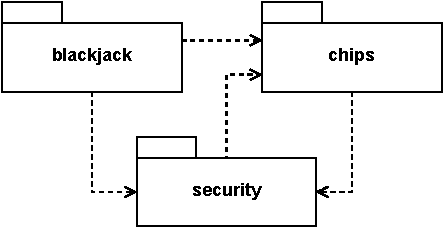
\includegraphics[width=.6\linewidth]{uml-casino-component-packages}
    \caption{Een UML-packagediagram van de logische componenten binnen het casinoproject.}
    \label{fig:uml-casino-component-packages}
\end{figure}

Vaak kun je fysieke componenten aanwijzen op basis van de herkende logische componenten.
Dit zijn componenten die niet alleen logisch samenhangen, maar ook als zodanig 
gerealiseerd (kunnen) worden. Vaak kan een fysieke component (met wat kleine aanpassingen)
aangeboden worden als zelfstandige Java-package, -module of -applicatie.
Een fysieke component biedt een manier aan om ermee te praten 
(een \emph{provided interface}, ook: \emph{componentfacade}).
Dit is een verzameling aan services, exceptions en \emph{data transfer objecten} (\emph{DTOs}) 
om met het component te praten.

Het is de bedoeling dat andere modules binnen het systeem alleen via deze 
provided interface praten met het component en niet de interne klassen rechtstreeks aanspreken.
Dit noemt men de \textit{facade convention}.
Het is een voorbeeld van \emph{implementation hiding} door middel van \emph{abstractie}.
Er is dus een soort inkapseling van klassen binnen de package van een component,
terwijl er alleen met de provided interface (de facade) gepraat wordt.

Om componenten van elkaar los te koppelen, proberen we binnen een component 
dan ook niet afhankelijk te zijn van de (interne) domeinobjecten van een andere component.
We kunnen daarvoor in de applicatie-laag met basistypen of DTOs te werken als vertalingsslag tussen 
het domein en de buitenwereld. Op die manier koppel je niet de buitenwereld aan de 
interne toestand van zo'n component. Als we naar het Chips-component kijken, 
zien we dat de componentfacade bestaat uit de ChipsService en een Balance. De ChipsService biedt 
de use cases aan van de Chips-component, terwijl de Balance een \emph{data transfer object} is 
met primitieve waarden.

De packaging binnen een component vindt plaats op basis van de functionele samenhang,
terwijl de koppeling slechts plaatsvindt tegen de klassen van de provided interface.
Dit kan bijdragen aan het bereiken van \emph{high cohesion} en \emph{loose coupling}.
De provided interface kan aangeroepen worden door een andere component,
een framework of een extern systeem. 
Zoals in Figuur~\ref{fig:uml-chips-component} is te zien,
worden de in de Chips component van het casinoproject de use case-gerichte,
taakspecifieke diensten geboden door (onder andere) de ChipsService.

Soms moet een component ook praten met andere modules of externe systemen. 
Dan biedt een component een \emph{required interface} (ookwel: \emph{componentgateway}) aan.
Dit is vaak een beschrijving van diensten die het component af wil nemen,
bijvoorbeeld van een ander component, een framework of een extern systeem.
In Figuur~\ref{fig:uml-chips-component} kunnen we zien dat de Chips component
diensten nodig heeft die zijn gedefinieerd in de ChipsRepository. Dit zullen diensten
zijn die te maken hebben met het opslaan van Chips. Dit wordt vaak ingevuld door een 
framework of library. In het casinoproject is dat een interface van Spring JPA.

\begin{figure}[H]
    \centering
    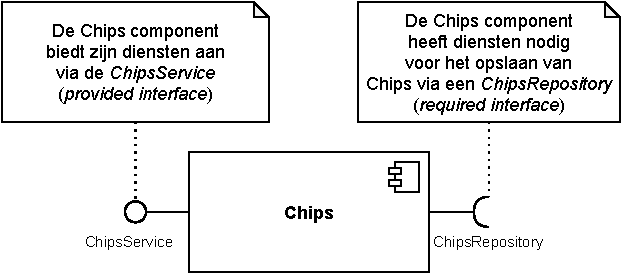
\includegraphics[width=.7\linewidth]{uml-chips-component}
    \caption{Een UML-componentdiagram van de \emph{Chips component}.}
    \label{fig:uml-chips-component}
\end{figure}

\newpage
In Java en andere object-georiënteerde talen 
zal je bij een required interface vaak een interface of abstracte klasse gebruiken.
Deze geeft aan met (abstracte) publieke methoden welke functionaliteiten vereist zijn.
Een implementerende klasse kan, door de interface te implementeren of de abstracte klasse te extenden,
aangeven dat het de benodigde functionaliteit aanbiedt in diens publieke methodes.
Het achterliggende mechanisme hiervoor is \emph{polymorfisme}.
De belofte is dat een component in zijn geheel vervangen kan worden. 
Het vervangend component moet dan wel voorzien in de vereiste functionaliteiten 
(\emph{required interface}).

\subsubsection{Wat zijn de components binnen het casinoproject?}
Hoewel we in dit project minder strikt omgaan met typische regels
voor fysieke componenten,
zou je van de structuur van het casinoproject een UML-componentdiagram kunnen maken 
zoals te zien in Figuur~\ref{fig:uml-casino-components}.
De controllers (\emph{provided interfaces}) zijn bedoeld om door Spring te 
worden aangeroepen wanneer een bepaald web request moet worden afgehandeld,
terwijl de repositories (\emph{required interfaces}) zijn bedoeld om door Spring 
te worden geïmplementeerd op basis van de benodigde opslagbehoeften.
Ook worden er application services aangeboden (\emph{provided interface})
die zowel aangeroepen worden door de controllers van de component zelf als door 
de application services van andere components.

\begin{figure}[H]
    \centering
    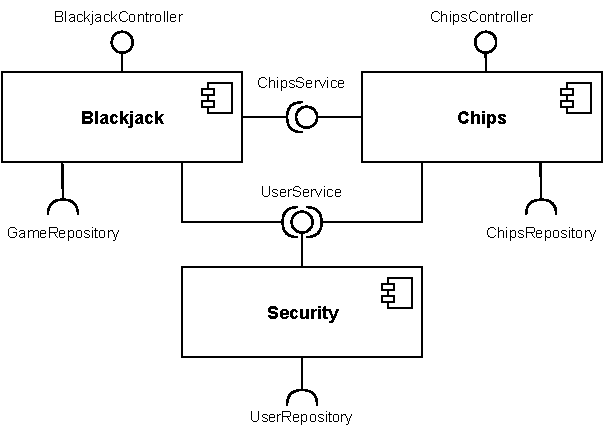
\includegraphics[width=.7\linewidth]{uml-casino-components}
    \caption{Een UML-componentdiagram van het casinoproject.}
    \label{fig:uml-casino-components}
\end{figure}

\newpage
\subsection{Lagen}
\index{gelaagde architectuur}
\index{laag}
Een applicatie, of een deel ervan, is vaak opgedeeld in lagen die 
elk verantwoordelijk zijn voor een ander soort logica binnen het systeem.
Het afhandelen van gebruikersinteractie 
is bijvoorbeeld iets heel anders dan het uitdelen van kaarten in een
kaartspel of het opslaan van een speelronde.
Een gelaagde structuur helpt niet alleen met het terugvinden van
bepaalde klassen op basis van het soort logica dat het betreft. Bij een 
losgekoppeld ontwerp kunnen lagen of onderdelen ervan gemakkelijk uitgewisseld worden.

\begin{figure}[H]
    \centering
    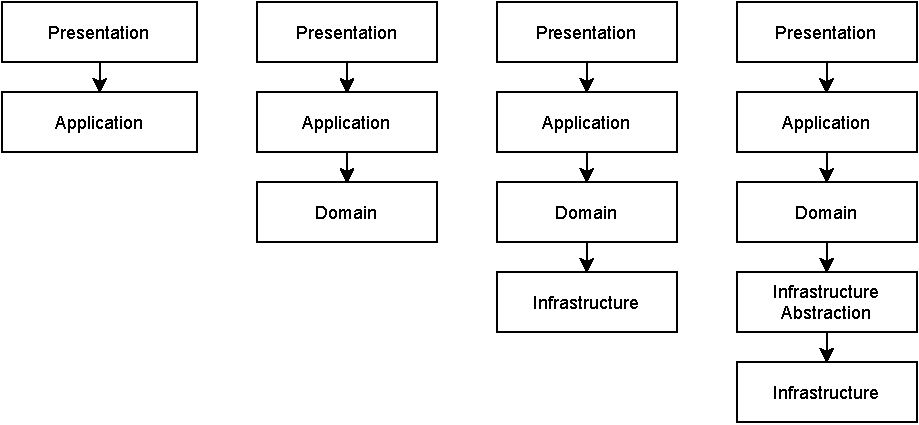
\includegraphics[width=.8\linewidth]{logical-layers}
    \caption{Voorbeelden van logische lagenmodellen met verschillende hoeveelheden lagen, waarin 
    verschillende soorten logica zitten.}
    \label{fig:logical-layers}
\end{figure}

Gelaagde architecturen komen in verschillende soorten en maten. Sommige applicaties 
zijn eerst opgesplitst in componenten en vervolgens ingedeeld in lagen. Andere zijn 
eerst opgesplitst in lagen, waarin vervolgens losse componenten zijn te bespeuren.
Het aantal lagen kan variëren tussen de twee en vijf lagen. Dit hangt af 
van de verschillende soorten logica en de specifieke architecturele eisen
van de onderdelen binnen een project. Hierbij kan je denken aan de soorten 
logica uit Tabel~\ref{table:logica-in-lagen}, gebaseerd op \cite{Pruijt2010}.

\begin{table}[H]
\centering
\begin{tabularx}{\textwidth}{|>{\raggedright}l|>{\raggedright\arraybackslash}X|}
\hline
\textbf{Logicalaag} 
    & \textbf{Verantwoordelijkheid} \\
\hline
\textit{Presentatielogica}
    & Het opbouwen en onderhouden van communicatie 
    met de gebruiker. \\ 
\hline
\textit{Taakspecifieke logica} 
    & Het coördineren van taakuitvoering en 
    het afhandelen van taakspecifieke functionaliteit. 
    In een bijbehorende laag zitten meestal applicatieservices die use cases 
    omzetten naar domeinacties met behulp van infrastructuurabstracties.
    Meestal geeft een applicatieservice een DTO terug. \\
\hline
\textit{Domeingenerieke logica}
    & Het leveren van generieke functionaliteit die te maken heeft 
    met het interessegebied van de business. 
    Domeinconcepten, business rules en entiteiten vind je vaak in lagen 
    met deze verantwoordelijkheid. \\
\hline
\textit{Infrastructuurabstractie logica}
    & Het vertalen van functionele (technologie-onafhankelijke) 
    vragen in technologieafhankelijke vragen aan de infrastructuur. 
    Hierin zitten meestal interfaces of abstracte klassen die door
    infrastructuurklassen moeten worden ingevuld (\emph{gateways}). \\
\hline
\textit{Infrastructuurlogica}
    & Het leveren van breed herbruikbare, niet businessspecifieke diensten, 
    zoals data persistentie, security, logging, deployment, etcetera. \\
\hline
\end{tabularx}
\caption{Typische soorten logica die men in aparte lagen kan aantreffen.}
\label{table:logica-in-lagen}
\index{logica in lagen}
\index{presentatielogica}
\index{taakspecifieke logica}
\index{infrastructuurabstractie logica}
\index{infrastructuurlogica}
\centering
\end{table}

\subsubsection{Regels}
Zoals er voor components geldt dat 
aanroepen naar binnen toe via de \emph{provided interface} moet gebeuren 
en aanroepen naar buiten toe via de \emph{required interface} moet gebeuren,
zo gelden er voor lagen ook vaak regels. In het geval van 
lagen zijn deze gebaseerd op het soort logica of het abstractieniveau.

Een veelvoorkomende regel is dat de afhankelijkheden enkel mogen plaatsvinden 
van hoger gelegen lagen naar lager gelegen lagen en niet andersom. 
\emph{Back calls} zijn niet toegestaan. \index{back call}
Een alternatief voor deze regel is dat afhankelijkheden enkel van buiten naar binnen
mogen lopen: van een flexibele infrastructuur (presentation en persistentie) 
naar een stabiele kern (business logic). Vaak kan je afhankelijkheden omdraaien door 
een interface of abstracte klasse tussen lagen op te nemen.

Een andere regel die je in strict layered architectures tegenkomt is dat 
afhankelijkheden geen lagen mogen overslaan. \index{strict layered architecture}
\emph{Skip calls} zijn dan niet toegestaan: \index{skip call}
tussen een hoger gelegen laag en een lager gelegen laag 
mag er alleen een afhankelijkheid zijn als er in de bedoelde
architectuur geen andere laag tussen hoort te zitten. 
Bij een drielagenarchitectuur (bijvoorbeeld: presentatie, domein, data)
mogen klassen in de presentatielaag dan niet rechtstreeks praten 
met klassen in de datalaag. Daar moet een afhankelijkheid op een
domein-module tussenzitten. Dit is vaak ook op te lossen door een tussenliggende 
interface op te nemen. De reden om dit op deze manier in te richten is om 
de koppeling tussen lagen te reduceren en het makkelijker te maken lagen (of delen daarvan)
makkelijk en flexibel inwisselbaar te maken. In relaxed layered architectures 
kom je deze regel overigens niet tegen. \index{relaxed layered architecture}

\subsubsection{Hoeveel lagen heeft het casinoproject?}
In het casinoproject is binnen components vier soorten logica te onderscheiden, 
aangewezen met packages, zie Figuur~\ref{fig:uml-casino-physical-layers}.

\begin{figure}[H]
    \centering
    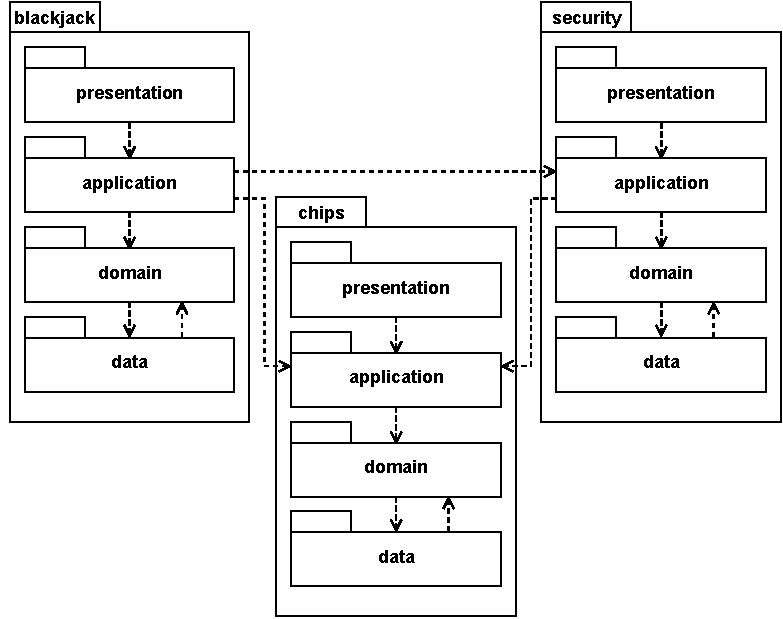
\includegraphics[width=.6\linewidth]{uml-casino-physical-layers}
    \caption{Components en layers kunnen met packages worden aangewezen binnen het casinoproject.}
    \label{fig:uml-casino-physical-layers}
\end{figure}

Deze packages corresponderen met de volgende soorten logica:
\begin{itemize}
    \item \emph{Presentation}: Presentatielogica. In het geval van een back-end API tref
    je hier alles aan dat hoort bij de technische vertaling van web requests naar Java-code. 
    Controllers (web request handlers) worden aangeroepen door het Spring framework 
    zodra een HTTP-request binnenkomt met een gedefinieerde route (HTTP-method + URL).
    \item \emph{Application}: Taakspecifieke logica. Hierin zitten applicatieservices (\emph{facades}) 
    die use cases omzetten naar domeinacties met behulp van infrastructuurabstracties. Een applicatieservices
    ziet vaak op één centraal domeinobject dat is opgebouwd uit of verwijst naar andere domeinobjecten.
    Door een applicatielaag in te richten kan dezelfde logica geboden worden onafhankelijk van de gebruikte 
    technologie in de presentatielaag: command line commando's, GUI's, web controllers of message handlers.
    \item \emph{Domain}: Domeinlogica. Domeinconcepten, business rules en entiteiten vind je vaak in lagen 
    met deze verantwoordelijkheid.
    \item \emph{Data}: Infrastructuurabstractie. Hierin zitten meestal interfaces of abstracte klassen die door
    infrastructuurklassen moeten worden ingevuld (\emph{gateways}). De daadwerkelijke infrastructuurlogica 
    wordt in het casinoproject ingevuld door het Spring framework.
\end{itemize}

Het casinoproject is dus opgezet met vier soorten logica in gedachten. Als je het 
lagenmodel echter strikt zou toepassen op Figuur~\ref{fig:uml-casino-physical-layers}, 
zie je een overtreding in de laatste twee lagen van elk component. 
De datalaag bestaat weliswaar slechts uit interfaces die door 
Spring geïmplementeerd worden, maar ze zijn afhankelijk van entities die
gedefinieerd zijn in het domein. Logisch gezien zou je het project daarom 
eerder beschouwen als een drie-lagen-architectuur. De laatste laag zou dan zowel
domeinlogica als infrastructuurabstracties bevatten. De laatste laag is opgedeeld 
in twee Java packages om de abstracte kern te scheiden van concrete 
aansluiting met infrastructuur. Het casino-project kent verder 
een relaxed layered architecture: je mag lagen overslaan.
Zo mag je in de presentatielaag een domeinobject teruggeven,
zodat het in een HTTP-response kan worden opgenomen.

\begin{figure}[H]
    \centering
    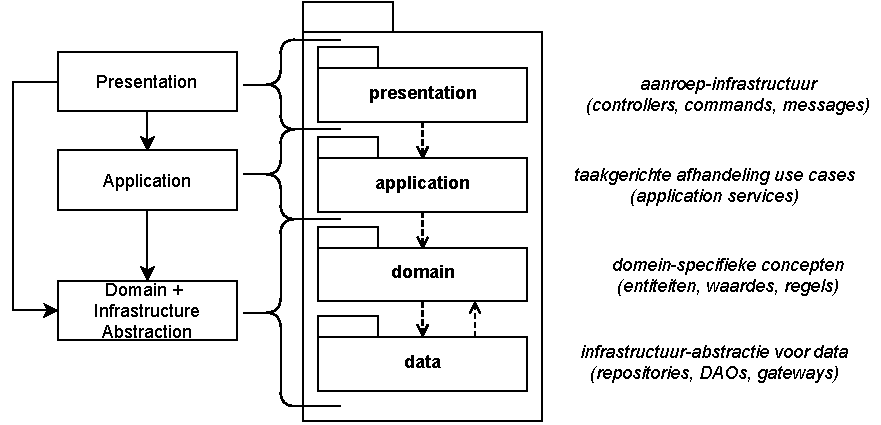
\includegraphics[width=.7\linewidth]{casino-layers}
    \caption{Het logisch en fysiek lagenmodel binnen de componenten van het casinoproject.}
    \label{fig:casino-layers}
\end{figure}

Als je het de realisatie meer wil afstemmen op de laging, zou je de 
entiteiten als losse objecten opnemen in de datalaag (als een soort DTOs) 
en een vertaalslag aanbieden tussen domeinobject en DTO. Als je daarnaast 
wil verbieden dat er lagen worden overgeslagen, zou je ook een vertaalslag 
kunnen toevoegen tussen DTO en domeinobject in de applicatielaag.
Als alternatief zou je de infrastructuur-abstractie
(de repository) kunnen opnemen in het domein en dat \textit{data} package verwijderen.
In ons project passen we deze regels echter niet zo strikt toe:
we accepteren een lichte koppeling op het framework en op ons domein.

\subsection{Subsystemen}
\index{subsysteem}
Binnen een \emph{subsysteem} kan je modules groeperen die binnen 
een laag (of component) bij elkaar horen, maar waar verder geen 
regels voor gelden. Dit is erg handig om grote projecten nog verder 
te organiseren. Je kan ervoor kiezen om subsystemen in te richten op 
basis van de technische rol die een groep modules vervuld, maar het is 
vaak mooier om ook hier aan te sluiten bij stukken samenhangende functionaliteit.
Zo kan je bijvoorbeeld binnen een domein 
(\emph{blackjack}: de logica om een blackjack spel te spelen)
een deelonderwerp aangeven 
(\emph{cards}: alles dat met kaarten te maken heeft).

\section{Packagestructuur in Java}
\index{packagestructuur}
Hiervoor hebben we het vooral over het modelleren van de conceptuele
en fysieke structuur van onze softwaremodules gehad, maar hoe kunnen we 
dit onderbrengen in onze code?

In Java kunnen we modules groeperen door gebruik te maken van 
\emph{packages} (in C\# en andere talen met \emph{namespaces}).
De naam van een Java-package lijkt op een soort omgekeerd webadres
en komt overeen met de onderliggende mappenstructuur.
Het is gebruikelijk om in Java-packages eerst te beginnen met de organisatienaam,
bijvoorbeeld \texttt{nl.hu.bep2}, en vervolgens de projectnaam \texttt{casino}.
Dan kunnen we het project opdelen in componenten, zoals in het casino-project: 
\begin{itemize}
\item \texttt{nl.hu.bep2.casino.chips}
\item \texttt{nl.hu.bep2.casino.security}
\item \texttt{nl.hu.bep2.casino.blackjack}
\end{itemize}

Binnen elke component kan wederom met packages 
onderscheid gemaakt worden naar 
het soort logica volgens een gelaagde aanpak. 
Dat leidt bij het casino-project tot de volgende 
mappen- en packagestructuur onder \texttt{src/main/java}:

\dirtree{%
    .1 nl.hu.bep2.casino.
        .2 chips.
            .3 presentation.
                .4 controller.
                .4 dto.
            .3 application.
            .3 domain.
                .4 exception.
            .3 data.
        .2 security.
            .3 presentation.
                .4 controller.
                .4 dto.
                .4 filter.
            .3 application.
            .3 domain.
            .3 data.
        .2 blackjack.
            .3 (...).
}

Als alternatief zouden we de (fysieke) componenten kunnen samenbrengen in 
modules in de zin van het Java Module System dat in Java 9 is geïntroduceerd.
Daaraan kunnen we extra regels koppelen rondom provided en required interfaces.
Daar is in het casinoproject echter niet mee gewerkt.

\section{Een voorbeeldflow}
Hoe loopt de flow binnen deze lagen? Laten we daarvoor een blik werpen 
op de \emph{deposit use case} van het Chips-component. 
Zie Figuur~\ref{fig:chips-sequence-diagram}.

\begin{figure}[H]
    \centering
    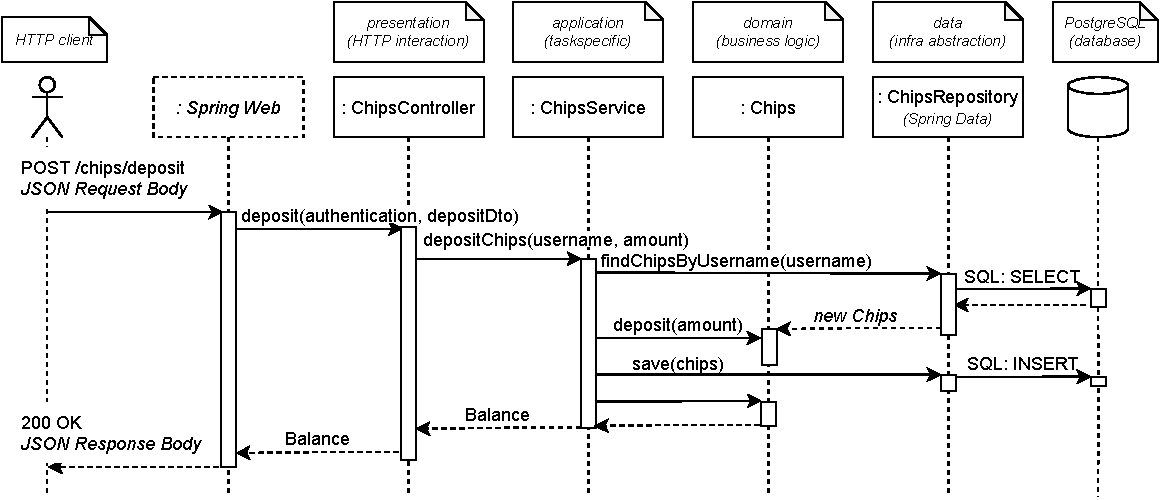
\includegraphics[width=\linewidth]{chips-sequence-diagram}
    \caption{De flow voor de deposit use case van het Chips-component}
    \label{fig:chips-sequence-diagram}
\end{figure}

Allereerst moet een HTTP-client een POST-verzoek doen naar 
\texttt{/chips/deposit}. We willen namelijk een overmaking toevoegen
aan de chips resource voor de huidige gebruiker. In dat POST-verzoek 
wordt de huidige gebruiker meegegeven via een JWT-token in de Authorization header
als deze is ingelogd. Vervolgens zet Spring Web dit verzoek om naar de bijbehorende 
controlleractie op de \emph{ChipsController} in de presentatielaag, met de
nodige informatie over de gebruiker (\emph{Authentication}) en de data die 
in de HTTP JSON Request Body zat (het \emph{Deposit} data transfer object).
De controller haalt de nodige data uit deze objecten en zet dit om naar 
een aanroep op de \emph{ChipsService} in de applicatielaag. Deze ChipsService
bevat allerlei methoden die de use cases van het Chips-component vertegenwoordigen.
De service roept de \emph{ChipsRepository} aan uit de datalaag om de hoeveelheid
\emph{Chips} op te vragen voor de betreffende \emph{User}. Vervolgens roept de 
service \emph{deposit} aan om de Chips om het aantal chips te verhogen met de 
gekozen hoeveelheid en wordt het \emph{Chips} object weer opgeslagen in de \emph{ChipsRepository}.
Ten slotte geeft de service een \emph{Balance} terug door de benodigde data uit het 
\emph{Chips}-object te halen en dit in een nieuw \emph{Balance}-object te stoppen.
De controller geeft ook deze \emph{Balance} terug aan Spring Web, waarop deze de 
\emph{Balance} omzet naar een HTTP JSON Response Body aan de hand van diens getters.

\newpage
\section{Samenvatting}
In dit hoofdstuk hebben we onderzocht op welke manier we een project kunnen 
indelen in modules ten behoeve van de onderhoudbaarheid ervan. We hebben 
kennisgemaakt met softwarearchitectuur en verschillende modulesoorten.

\begin{defbox}{Modulaire architectuur}
    Een modulaire architectuur is opgebouwd uit verschillende modules
    die elk hun eigen rol hebben binnen het gehele project.
    \newline\newline
    Fysieke \emph{componenten} zijn algemene groeperingen van deelfunctionaliteit
    die een \emph{provided interface} of \emph{componentfacade} aanbieden
    waar het component mee aangesproken kan worden. Ook kunnen ze 
    een \emph{required interface} of \emph{componentgateway} verlangen
    waarin de door het component benodigde diensten worden beschreven.
    Een component verbergt diens implementerende klassen. Daarom mag 
    er alleen via de provided interface met het component gepraat worden (\emph{facade convention}).
    \newline\newline
    Componenten kunnen worden ingedeeld in \emph{lagen} naar gelang het 
    soort logica dat daarin een rol speelt en in hoeverre een 
    onderliggende laag hergebruikt kan of moet worden. 
    Andersom kan een architect ervoor kiezen om lagen onder te verdelen in componenten.
    De aanroepen binnen een lagenmodel lopen alleen van boven naar beneden (\emph{back call ban}). 
    In een strikte laging mogen er geen lagen worden overgeslagen (\emph{skip call ban}). 
    \newline\newline
    Binnen componenten en lagen kunnen samenhangende modules in het algemeen worden
    aangegeven met \emph{subsystemen}. Dit is bijvoorbeeld handig voor het aanwijzen 
    van deelgebieden binnen een domein.
    \newline\newline
    Een onderhoudbare packagestructuur is begrijpelijk opgesteld, zodat je zaken kunt 
    terugvinden. Het helpt om aan te sluiten bij de bedoelde architecturele verdeling.
    \newline\newline
    Binnen het casinoproject is gekozen voor een indeling in componenten en lagen, 
    maar worden de regels minder streng gehanteerd. Het is bedoeld om te wennen 
    aan een modulaire opbouw. We accepteren een lichte koppeling op het framework en op ons domein.
\end{defbox}